\documentclass[tikz,border=5pt]{standalone}
\usepackage{pgfplots}
\pgfplotsset{compat=1.18}

\definecolor{corba}{HTML}{365FB3}
\definecolor{punt}{HTML}{C2415D}
\definecolor{guia}{HTML}{6B7280}

\begin{document}
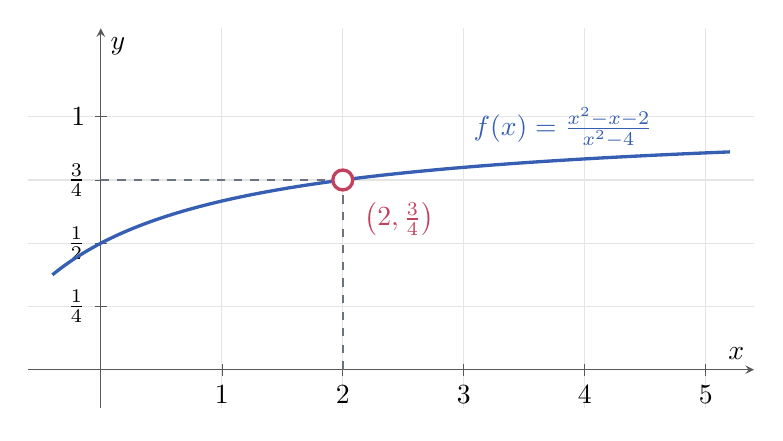
\begin{tikzpicture}
  \begin{axis}[
    width=10.8cm,
    height=6.4cm,
    axis lines=middle,
    xmin=-0.6,
    xmax=5.4,
    ymin=-0.15,
    ymax=1.35,
    xlabel={$x$},
    ylabel={$y$},
    xtick={1,2,3,4,5},
    ytick={0.25,0.5,0.75,1},
    yticklabels={$\frac14$,$\frac12$,$\frac34$,$1$},
    axis line style={black!65},
    tick style={black!65},
    grid=major,
    grid style={black!10},
    clip=false,
  ]
    \addplot[corba, very thick, domain=-0.4:5.2, samples=180]
      {(x+1)/(x+2)};

    \addplot[guia, dashed, thick] coordinates {(2,0) (2,0.75)};
    \addplot[guia, dashed, thick] coordinates {(0,0.75) (2,0.75)};
    \addplot[
      only marks,
      mark=*,
      mark size=3.6pt,
      punt,
      mark options={draw=punt, fill=white, line width=1.2pt}
    ] coordinates {(2,0.75)};

    \node[anchor=south west, text=corba]
      at (axis cs:3.0,0.84) {$f(x)=\frac{x^2-x-2}{x^2-4}$};
    \node[anchor=north west, text=punt]
      at (axis cs:2.1,0.70) {$\left(2,\frac34\right)$};
  \end{axis}
\end{tikzpicture}
\end{document}
